\chapter{Software základní desky}
Tato kapitola se zaměřuje na software základní desky PROTOPlantu a detailně popisuje jeho funkci.
Na software ostatních modulů se zaměřuje následující kapitola \ref{chap:moduleSoftware}.

\paragraph{Blokové schéma funkce softwaru základní desky}
Schéma funkce softwaru základní desky je shrnuto blokovým diagramem XXX.

\section{Sdílené knihovny}
Z~důvodu usnadnění programování základní desky i ostatních rozšiřujících modulů jsem vytvořil několik sdílených knihoven. 
V~nich je zahrnuto:
\begin{itemize}
    \item konfigurace systému
    \item nastavení jednotlivých pinů dle standardního rozložení, vč. možnosti nastavení vlastního
    \item práce s~displayem
    \item práce s~tlačítky
    \item řízení H-můstků
    \item ovládání senzorů
\end{itemize}
Díky těmto knihovnám je většina zdrojového kódu uložena v~nich. 
Koncový uživatel, který se rozhodne software modifikovat, poté pouze v~hlavním programu definuje, které moduly spustit a do konfiguračního souboru zapíše nastavení daných modulů.

\paragraph{Konfigurace softwaru}
Konfigurace softwaru pro jednotlivé verze hardwaru je řešena pomocí jednoho souboru.
Podle toho, jak jsou jednotlivá makra v~tomto souboru definována, prekompilátor následně sestaví software přímo pro danou verzi.
Část konfiguračního souboru je zobrazena níže.
V~této části lze nastavit parametry přístupového bodu Wi-Fi, který si PROTOPlant sám vytvoří, sériové linky a displeje.
\begin{lstlisting}
    //If wifi credentials not set OR wifi not found, 
    //create own AP with these credentials
    #define AP_SSID ProtoPlant
    #define AP_PASSWORD protoplant
    
    #define SERIAL_DEBUGGING    true
    #define SERIAL_BAUDRATE     115200
    
    #define DISPLAY_CONNECTED   true
    #define DISPLAY_ADDRESS     0x27
    #define DISPLAY_TIMEOUT     10000
    #define DISPLAY_COLONS      16
    #define DISPLAY_ROWS        4
\end{lstlisting}

\section{Datové sběrnice}
PROTOPlant primárně využívá dvě datové sběrnice:
\begin{itemize}
    \item I\superscript{2}C
    \item OneWire
\end{itemize}

\noindent\B{Sběrnici I\superscript{2}C} používá PROTOPlant pro komunikaci se zařízeními na stejné desce, případně pro řízení LCD displeje instalovaného na řídícím panelu (připojení přes PanCon). 

\subparagraph{Princip}
Na sběrnici je připojeno jedno zařízení jakožto master (řídící) a jedno či více zařízení jako slave (řízená).
Tato zařízení jsou navzájem propojena dvěma dráty (proto se I\superscript{2}C někdy přezdívá TwoWire), serial clock (SCL) a serial data (SDA).
Každé ze slave zařízení má sedmibitovou adresu (např. 0xE0), která musí být pro každé zařízení na jedné sběrnici odlišná.
Některá zařízení mají tuto adresu pevně zapsanou a nelze ji měnit, zatímco u~jiných ji lze změnit.
Zařízení připojené jako v~režimu master tuto adresu nepotřebuje, vzhledem k~tomu, že on sám vždy adresuje jen jedno ze zařízení.

\subparagraph{Komunikační protokol}
Za klidového stavu (neprobíhá žádná komunikace) jsou obě linky (SDA i SCL) připojeny nastaveny na HIGH.
Jakmile chce master zahájit komunikaci, vyšle takzvaný startovní signál, po kterém následuje adresa daného zařízení, jejíž nultý bit určí, zda chce master číst, nebo zapisovat.
Dále následují datové bity.
Jakmile jsou všechna data přenesena, vyšle master stop signál, čímž ukončí komunikaci a sběrnice se vrátí do klidu.
Rychlost celého přenosu určuje pulsování linky CLK.
Celý proces názorně zobrazuje obrázek \ref{fig:I2C-protocol}.

\begin{figure}[htbp]
   \centering
   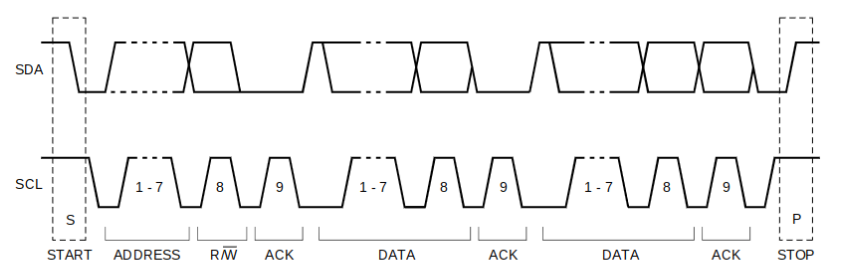
\includegraphics[width=\textwidth]{img/I2C.png}
   \caption{Celý datový přenos po I2C sběrnici. Převzato z~\cite{I2C_specs}}
   \label{fig:I2C-protocol}
\end{figure}

\paragraph{Sběrnice OneWire}
Sběrnici OneWire používá PROTOPlant pro komunikaci s~teplotními čidly DS18B20. 
Více o~této komunikační sběrnici v~\cite{DS18B20}.

\section{Komunikace mezi řídící jednotkou a jednotlivými moduly}
PROTOPlant podporuje dva režimy komunikace řídící jednotky s přídavnými moduly:
\begin{itemize}
    \item bezdrátová komunikace přes Wi-Fi
    \item kabelová komunikace přes UART (standard RS-485)
\end{itemize}

\section{Bezdrátová komunikace}
Je vhodná primárně pro malé skleníky v oblastech, kde nehrozí zarušení signálu.
Tento způsob komunikace je zatím stále ve vývoji.

\section{Kabelová komunikace a RS-485}
Kabelová komunikace probíhá přes tzv. UART (Universal Asynchronnous Receiver and Transmitter - univerzální asynchronní přijímač a vysílač).
PROTOPlant využívá průmyslový standard RS-485 umožňující komunikaci s~pomocí dvojlinky.
Opět je zde uplatněn princip master - slave (řídící jednotka je master, ostatní moduly slave).
Pro tento způsob komunikace existuje několik protokolů, pro příklad velmi často používaný ModBus, nebo nedávno vytvořený JANUS\cite{JANUS}, který používám. 
Více o~principu RS-485 a samotném protokolu v~\cite[21-25]{JANUS}

\chapter{Software dalších modulů}

\label{chap:moduleSoftware}
Software přídavných modulů je navržen tak, aby k~jeho běhu nebyl zapotřebí velký výpočetní výkon.
Obecně lze jejich funkci znázornit blokovým diagramem \ref{fig:PPCU-to-MODULE-communication}.

\chapter{Zvláštní stavy}
PROTOPlant má několik zvláštních stavů, ve kterých pracuje v omezeném režimu.
Tyto stavy slouží primárně pro zabránění poškození systému.

\paragraph{Režim nouzového chlazení}
\label{paragraph:CoolingMode}
Do tohoto režimu přejde systém v~případě, že teplotní senzor na základní desce PPCU detekuje přehřívání. 
Dojde k~automatickému vypnutí výstupů řídící jednotky.
Poté se systém restartuje, aby vyloučil chybu softwaru.
V~případě, že softwarovou chybu nedetekuje, vyčká, než se teplota sníží na běžnou provozní hodnotu, kterou průběžně vypočítává z~průměrů hodnot naměřených před prudkým nárůstem.
Po ochlazení systém pokračuje v~normálním chodu, ovšem na displeji zůstane upozornění, že k~chybě došlo.

\newpage